\chapter{Implementation}
\label{ch:implementation}

\section{Project Management}
The table below is the initial project timetable from the project specification document. It was used as a rough guide to keep the project on track by helping to know what tasks needed to be done and for how long.

\begin{table}[H]
	\begin{center}
		\begin{tabular}{ | c | l | }
			\hline
			\textbf{Dates} & \textbf{Event}                    \\ \hline
			T1 W1-2        & Project specification             \\ \hline
			T1 W1-2        & Research into development tools   \\ \hline
			T1 W3-9        & Development of website foundation \\ \hline
			T1 W4          & Design basic UI                   \\ \hline
			T1 W5-7        & User authentication               \\ \hline
			T1 W8-9        & Integration with PlaidAPI         \\ \hline
			T2 W1          & Testing of website foundation     \\ \hline
			T2 W2-10       & Repeated strategy development     \\ \hline
			Easter         & Finishing touches                 \\ \hline
			Throughout     & Document research                 \\ \hline
			T3 W1          & Dissertation due                  \\ \hline
		\end{tabular}
	\end{center}
	\caption{Initial project timetable \cite{ProjectSpecification}}
\end{table}

Following the submission of the progress report, it was made more evident that the project had four key phases instead. The first phase was research into the development methodologies and design. The second phase was the development of two proof-of-concepts and then merging them into a single application, following the waterfall methodology. The third phase was repeated strategy implementation and testing, following an agile methodology. The final phase was adding the budget prediction as a separate major feature. These divisions were a simple progression from the original timetable and were more natural with the whole project schedule by that point.

\subsection{Research and Design}
Most of the findings in this section have been outlined in the previous chapters, but it is still worth discussing how the research was conducted and the structure of this process. This phase was performed before the progress report and timetable change, so it aligns with the original project specification.

Initially, only the aim of the project and the plan to use open banking were set in stone. In early term 1, research into how open banking is performed and how a developer can utilise the service was the main priority, this is when the discovery of Plaid was made, and the decision to use it occurred. With familiarisation and proficiency in Next.js, it was a clear choice to use as the framework, and many of the other design decisions were made after understanding how to use Plaid.

\subsubsection{Research Methodology}
Plaid is a relatively new technology, but it is still like any framework, so a standard research methodology was used to understand how to use it. Vinicius' article \cite{FrameworkLearning} talks about the best approach for learning a new language or framework and has almost ten thousand claps (the measure of Medium's popularity), so many others agree. The article is a good summary of the whole process. The main points that were followed when learning Plaid are: start with the basics, read lots of documentation, find examples on GitHub and Stack Overflow, and finally, build something. In addition, due to Plaid's YouTube channel \cite{PlaidYouTube}, watching videos was also included because it provided an effective way to learn.

Plaid has a `getting started' video which helps explain the service's basics and the terminology used in the documentation. Following this, the Plaid documentation was read to understand the service's architecture and how it works. In addition, learning its features helped identify what features could be added to the application to improve financial capability. Unfortunately, due to the recency of the revised architecture of Plaid, there were few examples of how to use it on GitHub and almost no questions on Stack Overflow; however, as part of the Plaid getting started video, they provide a code repository with a basic implementation of Plaid that helped to understand the service.

Learning to use Plaid helped inform many other design decisions; for example, the Plaid authentication flow dictates the need for separate frontend and backend services to be developed and a database to store the users' credentials.

\subsubsection{Other Technologies}
The other major development technologies researched here included Next.js features that the developer had not used before, such as server-side rendering; the combination with TailWindCSS; and the use of PocketBase. The research method into these technologies was similar to when learning Plaid, as it had proven effective. The main difference is that more documentation and resources were available, making learning slightly easier. As well as technologies, new concepts had to be learnt, such as how authentication should be performed to ensure that user information is kept secure and how to follow modern web development best practices to build a successful web application.

The final point in Vinicius' article was to build something. This is the primary reason for the project's next phase of building two proof of concepts. It was to test and improve the knowledge of the technologies and concepts learnt, but also provided a reasonable basis for the actual application itself.

\subsection{Proof of Concepts}
To put the research from the previous phase into practice and work with the new technologies, this phase was building two separate proof of concepts, one to have basic user authentication and the other to be able to interact with the Plaid API. After building both prototypes, they were merged into one application, forming the basis for the rest of the project.

This implementation phase was the first deviation from the original plan in the specification. In this instance, the development followed the waterfall methodology. This is because it lends itself nicely to how this phase is structured. A clear step-by-step plan was constructed with the knowledge of what the technologies can do and a clear goal for each proof of concept. In addition, there was only one developer, so the waterfall methodology was an excellent way to ensure that the project stayed on track and that the developer was not overwhelmed with too many tasks.

\subsubsection{Waterfall Methodology}
Waterfall is known for being effective in projects with concrete objectives. Both applications were worked on simultaneously, performing each stage of the waterfall process for both applications. This was done to ensure that the applications could interact with each other when the time came to merge them. For example, the second stage of the methodology is designed, so both the applications' designs were set out simultaneously and both before the implementation (the next stage).

This sequential process is easy to manage but performs poorly for unexpected changes. This meant that the original requirements had to be detailed enough to encompass any possible queries, as well as have contingency plans in place. For example, from some initial research, some of Plaid's endpoints could take in an array of accounts and return the transactions for all of them; however a user on an online forum had mentioned that this often fails. The prioritised plan was to use this Plaid endpoint; however, if it did not work, there was also a plan and design to iteratively query a different endpoint for each account, which would functionally be the same.

\subsubsection{User Authentication}
User authentication is needed to allow only logged-in users to access their dashboard, and only each logged-in user can access the transactions for the access tokens they created. The design for this application was to have three pages. The first page is the signup page, where they can create an account. The second page is the login page, where they can log in to their already-created account. The final page is the dashboard which displays the user's email if logged in and redirects to the login page if they were not. The signup and login pages have links for users to navigate between them.

The implementation of user authentication is simple yet secure. The signup and login pages have two inputs for the email and password and a submit button for the form. When a user creates an account, the client first checks that the email is valid and unique and that a password has been entered. If so, the database is populated with the new account and the user is sent to their dashboard. The user is notified via an error message if the email is not valid or unique. The PocketBase npm package is used to make the appropriate calls when creating the account or logging in. In addition, this package automatically hashes and salts the passwords for security.

The login page works similarly, but instead of creating a new account, it checks that the entered email and password match an account in the database. If so, the user is sent to their dashboard; if not, they are notified of the error via a message on the page. On the dashboard page, the user is checked to be logged in via the PocketBase authStore, which uses JSON Web Tokens (JWT) under the hood. Using these tokens means they can hold the user's ID and allows the database to limit access to the user's data by only allowing requests from that user. The ID is encrypted in the JWT, which itself is stored in a cookie. In addition, the JWT is only valid for a short period to avoid cases where the cookie is stolen, and the user's account can be accessed by  else. Security is a major concern for this project as it handles sensitive financial data.

\begin{figure}[H]
	\centering
	\includegraphics[width=\textwidth]{images/signup_page.png}
	\caption{Minimal Signup Page for the User Authentication}
	\label{fig:Signup_page}
\end{figure}

\begin{figure}[H]
	\centering
	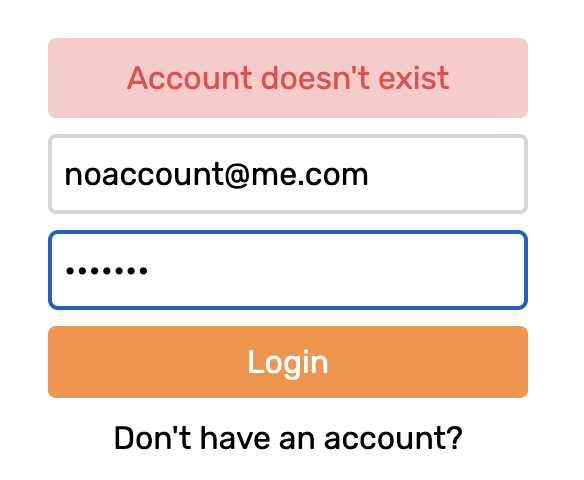
\includegraphics[width=0.5\textwidth]{images/no_account.png}
	\caption{Login Component, with an Example Error Message}
	\label{fig:Login_component}
\end{figure}

\begin{figure}[H]
	\centering
	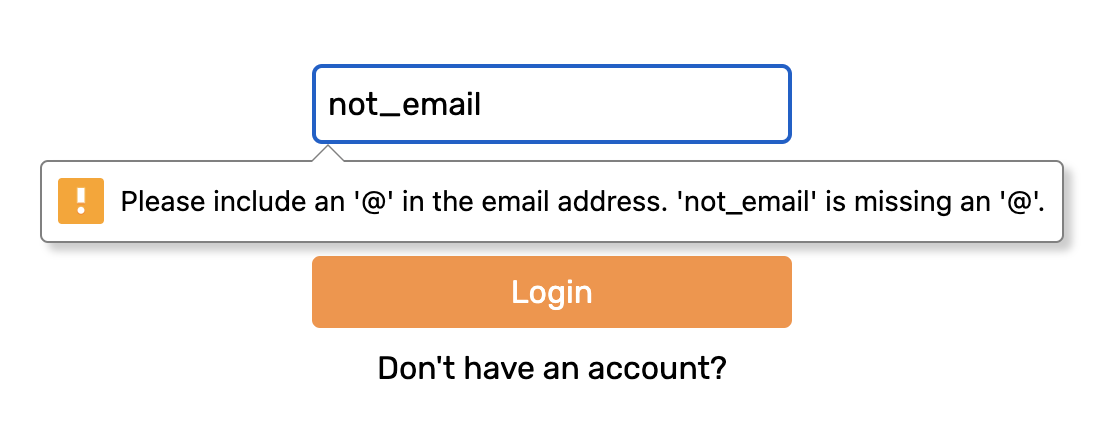
\includegraphics[width=0.9\textwidth]{images/email_validation.png}
	\caption{Client-side Validation for the Email Input}
	\label{fig:Email_validation}
\end{figure}

\subsubsection{Plaid API}
The second proof of concept was to be able to interact with the Plaid API. The design allows a user to follow the authentication flow of Plaid in linking a bank account and getting the resulting access token. Then, with this token, access their recent transactions. To begin the process, a user clicks on a button to request the link token and has the link widget pop-up. The rest of the authentication flow is as described in the background section (\ref{sec:plaid-authentication-flow}), and after linking, the access token is just stored client-side at this stage.

This system required minimal design and little styling as the authentication flow was already decided. This proof of concept was aimed at having functionality, so there was no need for fancy-looking components. Again, as using the waterfall methodology, the implementation was also simple. From the previous research, the whole process was already known, so there was little deviation from the complete plan created in the previous phase.

\subsubsection{Merging}
At this stage, there were two independent proof-of-concepts that served different purposes; however, the project needed to have one working application that does what both of them do and more. Both the proof-of-concepts had been written using git but were on separate branches. The basic user authentication was deemed more fragile, so the Plaid interaction was decided to merge into that application. The idea was to have the user perform the basic authentication; then they can link their bank accounts on the dashboard, and each access token generated is stored in the database. Furthermore, if that user already had an access token available, then on the dashboard, they can request their transactions, which are displayed in the console.

With the waterfall methodology and knowing how to implement these systems independently, each stage was meticulously planned. Hence, the merge went smoothly, and the bare-bones application was ready to add the strategies. The only new feature, not in either, was the ability to store the access token in the database and retrieve it when doing the transaction query. It was similar to performing basic user authentication, such as getting a user's email, and there were many resources online to help. This aspect was added as a feature branch and then merged into the main branch to follow the idea of GitHub Flow explained below (\ref{sec:github-flow}).

During the implementation, something that was not considered was when a user has multiple access tokens and what to do. This oversight was easily mitigated, as the rest of the functionality was implemented per the original plan, and then, only after this was completed, the new feature was added. The slight modification was made so that when requesting the transactions, instead of getting the first access token, it returns all the access tokens, and then for each, a query is made to Plaid. This differs from a user with several linked bank accounts, as each access token can contain multiple bank accounts. However, at this point, the ability to toggle the individual bank accounts was not worried about.

\subsection{Repeated Strategy Implementation}
By this stage, the application was elementary and only could link bank accounts and retrieve transactions. The actual strategies to help improve financial capability were yet to be added or even designed. This was a separate major phase in the project, and instead of using the waterfall methodology, an agile methodology was more appropriate and so used. It was not any particular sub-methodology like scrum or lean, but instead just had very agile practises and was worked on in sprints. Each sprint was for a different strategy, so they were independently added but came together to form the final application. This separation was also shown during development as each strategy was implemented on a separate branch and then merged after passing the tests and being mostly complete.


\subsubsection{Agile Development}
Generally, the waterfall methodology should be prioritised for a project of this scale, especially where there is only one developer. However, agile was more appropriate for the repeated strategy development due to the requirements being challenging to define prior to each strategy. Each strategy, and therefore sprint, contained research into how best to include the strategy to maximise financial capability. This meant that the actual plan for each strategy was not known until the research was complete, therefore it was difficult to set clear objectives needed for waterfall. Similarly, agile allowed for each sprint to consist of this research, but then followed by the design and implementation. If any issues arose during the implementation, they were easily managed by altering the design, if appropriate, due to the flexible nature of agile.

Initially, it was decided that each sprint would be three weeks long, one week each for research, development, and testing. However, it was found that this gave too much time for each section, especially for research, so it was modified accordingly. Agile's ability to change on the fly was a significant benefit, particularly for this example. The sprint was reduced to roughly ten days, and there were no set periods for each section (research, development and testing); instead, the time was flexibly split among the three. This was useful after completing the transaction strategy and moving on to the categories strategy. Much less time needed to be spent on the research as there was some crossover, meaning more time was spent on the implementation and testing.

\subsubsection{Credential Management}
Following the merged proof of concepts, the application was sent to Plaid to request development access (instead of using sandbox mode). The application was approved thanks to the previous research and secure authentication flow, the application was approved. As outlined in the background section (\ref{sec:plaid-operation-modes}), development access means real live financial information can be accessed and used. This was a significant milestone, but it also came with further things to manage.

With development access, the application can have one-hundred access tokens in total. The limitation meant the credentials were treated as a resource and infrequently used to ensure enough were available for the final testing stages and the demonstration in the presentation. On top of this, all unit tests were only ever run in sandbox mode and only once these were passed did integration testing begin. Integration testing was first done in sandbox mode, but once happy, the same tests were performed in development mode. More often than not, no issues arose in development mode, but it was still essential to test in both modes to ensure the application's reliability.


\subsubsection{GitHub Flow}
\label{sec:github-flow}
As mentioned earlier, each strategy had its own branch and only merged once it was complete. This was an attempt to follow the GitHub Flow branching model \cite{GitHubFlow}. It involves having the main branch always deployable; all changes are made through separate feature branches via pull requests and merging; and rebases are used to avoid conflicts. The advantages include that multiple versions do not need to be managed, frequent changes can be pushed, e.g. after every sprint, and the codebase is much cleaner to work with.

The original plan was to use the GitFlow workflow \cite{GitFlow}, where there are develop and feature branches; however, this workflow is aimed at more collaborative projects and ones that need stable releases at set periods. Furthermore, GitHub Flow offered the same advantages for a single developer and was much less complex.

\subsubsection{MVP and Testing}
By the end of the repeated strategy implementation, a minimal viable product (MVP) was created that had the functionality to improve financial capability but still had room for additional features like budget prediction. Each component was thoroughly tested, as well as the integrations and pages as a whole. The individual component testing was often done in code and included the frontend as well as the backend, whilst the integration testing was mainly done manually. Some integration tests were completed in code, and all the automatic tests had to be passed before any branch was merged.

\subsection{Budget Prediction}
Following the repeated strategy implementation, there was a basic budgeting strategy; however, it only displayed the expenditure so far in the current month and allowed the user to set a budget. The original aim was to increase financial capability. A valuable feature that does this is predicting a user's expenditure and allowing them to adjust earlier, ultimately making better decisions.

Unlike the previous strategies, the budget prediction was added as a separate major feature because it was much more extensive. In addition, more research and planning were required as it involved creating machine learning models and a separate server to host the model. By this time, only minor tweaks were being made to the MVP as hotfixes, and the GitHub Flow workflow was followed again by performing this in a separate feature branch.

The process for this feature was somewhat treated like another agile sprint; however, it was not formalised like this. Going into the prediction, there was little certainty about how effective it would be or what the requirements were outside of predicting future expenses.

To manage this section, the machine learning models needed real financial data for training to be the most accurate. This has privacy concerns as the model learns from this data, so the resulting predictions can leak information. Furthermore, there was a limitation on the amount of real financial data accessible, so it was decided to mix the data. The model was trained using only the developer's financial data and some of the data from Plaid's sandbox mode. This was in an attempt to still create a useful model, but not leak any information and not overfit on a single individual. In addition, some data manipulation techniques outlined in the implementation were used to simulate more data and make the model more robust.

\section{Active Bank Accounts}
As part of the navigation bar shown in figure \ref{fig:DashboardNavigationBar}, the rightmost button with the label `accounts' is a dropdown. Clicking it displays a menu containing all the linked bank accounts, an add accounts button, and a logout button. Each linked bank account is a bar containing a toggle button, the name and type of the account, and a logo representing which bank chain it is from. The add accounts button allows users to link more bank accounts by beginning the Plaid authentication flow. The logout button lets the user log out, and the application will clear the cookie.

This functionality was implemented as part of the transactions sprint as it was not a part of the initial proof of concepts; however, it is necessary for all the other strategies. All the bank accounts are active by default; however, the user can toggle them off to exclude them from the analytics. Each bank account has an associated ID, so a list of active bank account IDs is stored as state in the navigation bar. This array is passed to each strategy component as a prop to filter the data and only include the active accounts.

\vspace{\baselineskip}

\begin{figure}[H]
	\centering
	\includegraphics[width=\textwidth]{images/accounts_dropdown.png}
	\caption{Account Dropdown Component for Sandbox Mode (left) and Development Mode (right)}
	\label{fig:AccountsDropdown}
\end{figure}


In figure \ref{fig:AccountsDropdown} above, the left image is from the sandbox mode, and the right image is from the development mode. In sandbox mode, only the savings accounts have been toggled on, for example, if a user wanted only to view the analytics for those accounts. In development, all the bank accounts, a Monzo and two Revolut accounts, are enabled. When switching between a toggled account, the icon has a slight animation, and when hovering over the account, the background colour changes to a light-grey.


\section{Strategies}
This section aims to outline the strategies that were implemented in the application. Therefore, only the final option decided in their respective design section will be explained. They were each implemented as independent sprints; however, they all aimed to improve financial capability by providing the user with information and tools to make better financial decisions.

\subsection{Transactions}
The transactions strategy was the first that was implemented, so there was a lot of experimentation and learning how best to get the data from Plaid, propagate it to the frontend, and then display it nicely.

Each strategy was implemented as a separate component, and the data required, such as the user object and active accounts, were passed down as props in the React model. This meant that the dashboard would render the component of the strategy currently being viewed.

The transactions strategy is implemented as a table where each row is a separate transaction to a merchant. The transactions are grouped by date and in reverse chronological order. When querying Plaid, it returns the transactions in the order of the accounts, so some extra data preparation was needed.

\subsubsection{Data Flow}
For this strategy, a single Next.js API route was required. It takes only the user ID as a parameter and queries the database for all the access tokens associated with that user. It can only see the access tokens that it created, so in this case, it would just get all the access tokens. With these, it requests Plaid to get the transactions for each access token. The transactions are then grouped and sorted in the API route so the frontend performs minimal work. The transactions are then returned to the frontend as a JSON object to be displayed.

\subsubsection{Plaid Endpoint Choice}
Plaid has multiple endpoints that access transactional data. To begin with, ``/transactions/sync'' was used, which gets the transactions. The first call returns all the historical transactions (up to a limit) along with a cursor; subsequent calls update the cursor and only return transactions from after the cursor. This reduces the data flow and means the transactions can be stored locally for faster loading. On strategy load, however, the UI needs to send two requests, one to the database to get the historical transactions and one to Plaid to get any since.

The Plaid API call ended up being changed to use ``/transactions/get'' instead, which returns the transactions between an input start date and end date. This was mainly because the transactions did not need to be stored, so it improved security. Plaid encourages the use of the ``transactions/sync'' endpoint as it acts as a subscriber model and also paginates the data; however, the get endpoint enabled code reuse for later strategies, withdrew the dependency on the database and also reduced the number of requests when loading the strategy.

\begin{figure}[H]
	\centering
	\includegraphics[width=\textwidth]{images/transactions_development.png}
	\caption{Transactions Strategy Component in Development Mode}
	\label{fig:TransactionsStrategy}
\end{figure}

The above figure (\ref{fig:TransactionsStrategy}) is an example of the transactions strategy with two separate bank accounts enabled in development mode. Each transaction has its own bar and displays relevant information to help provide an overview. In addition, income is coloured light-green, and expenditure is coloured light-red. Whenever a transaction is hovered over, it is coloured slightly darker as feedback. Often, there are enough transactions that vertical scrolling is required to view them all; however, there is no consistent way to style the scroll bar as it depends on the browser. To account for this, the scroll bar was removed entirely, but the bottom-most viewable transaction has an opacity gradient to indicate that more transactions are below.

\subsection{Categories}
The categories sprint followed naturally from the transaction sprint, as much of the backend functionality could be reused. For this strategy, only the expenditure needed to be analysed. One option was to modify the Next.js API route to automatically separate the data into income and expenditure (by positive and negative value). However, it would have involved some slight changes to the transaction strategy. So instead, a similar but new Next.js API route was created to get the expenditure data only. This also acted as an optimisation as the categories strategy only needed the previous thirty days of transactions, so it sped up the data processing by creating a different API route.

\begin{figure}[H]
	\centering
	\includegraphics[width=\textwidth]{images/categories_sandbox.png}
	\caption{Categories Strategy Component in Sandbox Mode}
	\label{fig:CategoriesStrategySandbox}
\end{figure}

The above figure (\ref{fig:CategoriesStrategySandbox}) is an example of the categories strategy component with four accounts enabled in sandbox mode. On the left is a dynamic pie chart that shows the relative amounts each category made up for the past thirty days. The colours are intelligently chosen; in the above example, there are four categories, so four colours that are the most distinguishable from each other are chosen. In the figure, the user is hovering over the light-blue section, 'Food and Drink', so the total for this section is displayed. On the right is the list of all expenditures for the past thirty days, but these are not grouped at all, and there is an emphasis on the category, unlike in the transactions strategy.

The below figure (\ref{fig:CategoriesStrategyDevelopment}) is an example of the categories strategy page in development mode with two accounts enabled. In this case, the pie chart is more realistic as it comprises real data. In addition, a filter has been applied to the categories to only show expenses in the 'Food and Drink' category. To apply this filter, the user has to click on the 'Food and Drink' category in the pie chart; to remove the filter, they can just click the red trash icon above the expenses.

\begin{figure}[H]
	\centering
	\makebox[\textwidth][c]{\includegraphics[width=1.05\textwidth]{images/categories_development.png}}
	\caption{Categories Strategy Page in Development Mode with a Filter}
	\label{fig:CategoriesStrategyDevelopment}
\end{figure}

\subsection{Budgets}
\label{sec:budgets}
There was no budget prediction in the original sprint for the budgeting strategy. Instead, the sprint resulted in a graphical view of the previous expenditure by displaying the amount spent each day, with a total amount on the side. The user can also enter an amount into the month's budget, which is also displayed on the line chart. The research portion of this sprint did identify that budget prediction is a valuable feature, but it was not considered at first because it involves more time than a single sprint. After the end of the investment sprint, the budget strategy seemed lacking, so a new phase was proposed to incorporate budget prediction.

\subsubsection{Time Series Forecasting}
As the design section (\ref{sec:BudgetPrediction}) mentioned, using a neural network was the best budget prediction option. The decision that was most key in turning the problem of budget prediction into a more well-defined problem was turning the expenditure data into cumulative amounts spent. This altered the data into a time series and meant that much more research and literature were available on tackling this problem. The cumulative amounts also were reset every month to match the budgeting period but made no difference to the predictions as the model learnt this.

The book Forecasting: Principles and Practice (3rd edition) \cite{ForecastingPrinciplesPractice} was a particularly useful resource for this section. It talked about the effects of seasonal time series, in this case, cumulative resets; how to apply linear regression techniques, which helped decide to avoid this; and using a neural network to make predictions.

\subsubsection{Long Short-Term Memory}
The term that repeatedly cropped up during the research was LSTM, meaning Long short-term memory. These are ``a type of recurrent neural network capable of learning order dependence sequence prediction problems'' \cite{LSTMGentleIntro}. The cumulative data could be seen as an order-dependent sequence, and the problem is just predicting the following value to appear in the sequence.

LSTMs differ from ordinary recurrent neural networks because the individual units have single-value memory cells that three gates can control. The first gate is an input gate determining if the cell's current value should be summed into memory. The second gate is the output gate which determines if the memory is added to the input as output. The final gate is the forget gate, determining whether memory should be cleared. Each gate has an associated weight learnt during training, like ordinary neural networks \cite{LSTMBig}.

\newpage
\subsubsection{Training}
As part of training the LSTM model, the input training data, consisting of the past three years of transactions, was first modified. The data was turned into the cumulative data and reset at zero every thirty days, but in addition, it was split in such a way as to maximise the amount that could be learnt. This was done by taking the first value up to the thirtieth value as one training example and the thirty-first value being the predicted output. Then taking the second value up to the thirty-first value as the following training example, the thirty-second value is the predicted output. This method is shown more clearly in the figure below (\ref{fig:TrainingData}) and resulted in 1064 training examples. Techniques such as test-train split and validation sets were also used.

\begin{figure}[H]
	\centering
	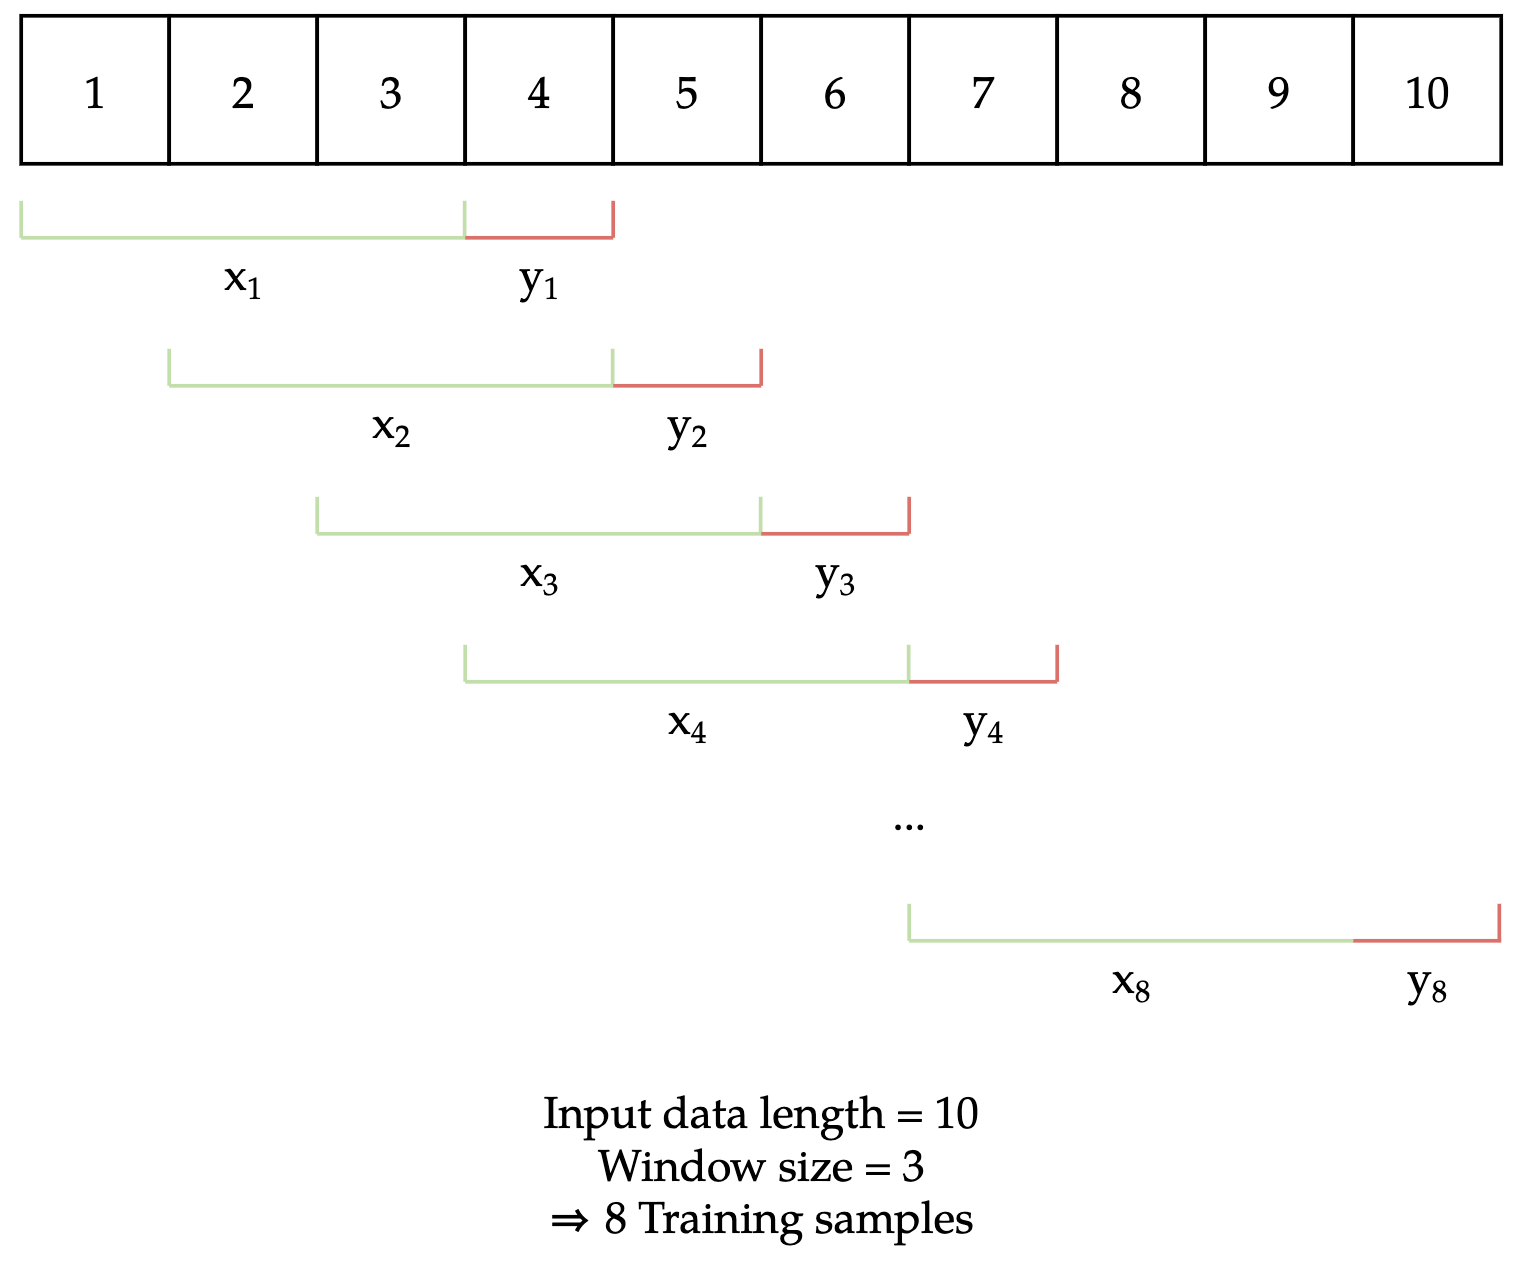
\includegraphics[width=\textwidth]{images/rnn_sample_generation.png}
	\caption{LSTM Training Data Generation}
	\label{fig:TrainingData}
\end{figure}

\subsubsection{Architecture}
Throughout the research and testing phase, LSTM models were the most accurate relative to other neural network architectures and machine learning models like linear regression. This also complimented the fact that there is support for LSTM models in the Keras library. The best structure of the network, which was found to be sufficiently simple that it could be trained in a realistic amount of time but also sufficiently complex to learn the data, was a single LSTM layer with 64 units, followed by a dense layer with 1 unit as output. Furthermore, to make the predictions realistic but not too overfit on the training data, 30 epochs were used to train the model. Finally, a window size of 30 was used, meaning the model has 30 inputs to match the modified training data and budgeting period.

\subsubsection{Results}
\begin{figure}[H]
	\centering
	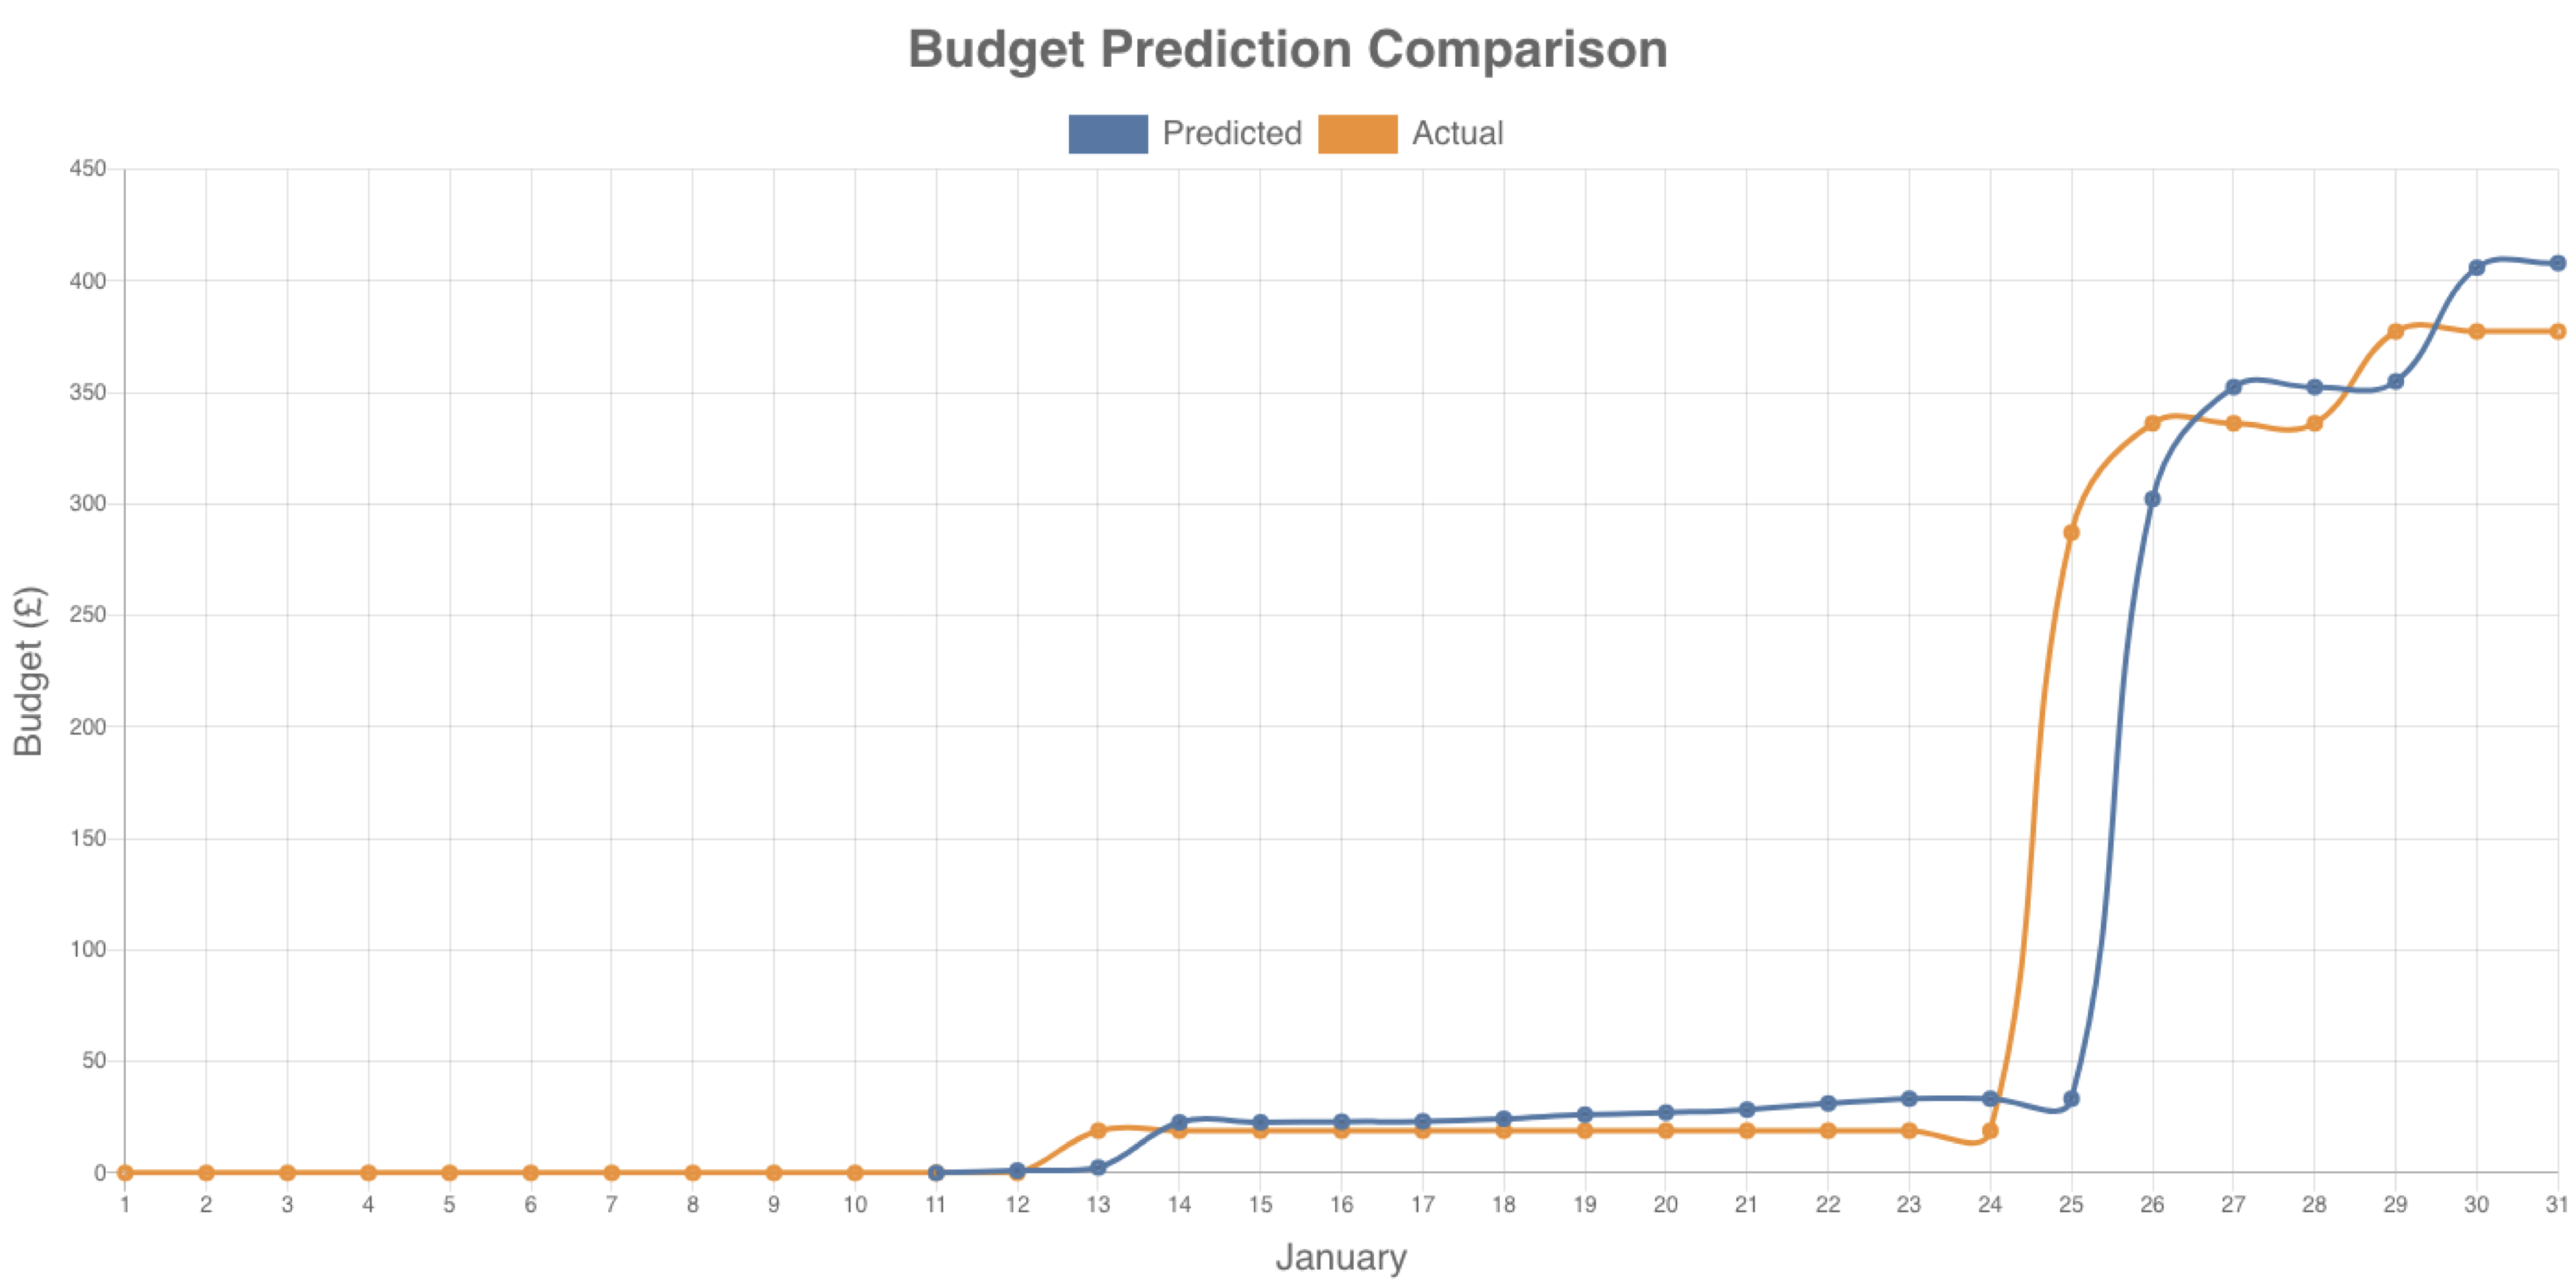
\includegraphics[width=\textwidth]{images/budget_prediction_comparison.png}
	\caption{Budget Prediction Analysis}
	\label{fig:BudgetPredictionResults}
\end{figure}

The above figure (\ref{fig:BudgetPredictionResults}) displays the difference between the predicted vs actual expenditures. In this instance, the data used for the graph is the fake data generated by Plaid, so it is not even related to the data on which the model was trained. Nevertheless, the model predicted the expenditure accurately and followed the pattern effectively. There is a slight offset in the two lines, but this was found to be due to how Plaid generates its transactions. They assume that each month has thirty days, but the graph is for January, which has thirty-one days, thus explaining the offset.

\subsubsection{Budget Strategy}
The accurate budget prediction model is incorporated into the budget strategy by making predictions for the remaining days of the month. For example, suppose the user is accessing the tool on the fifteenth day of the month. For the past fifteen days, the tool will have access to their actual transactions and can plot the cumulative expenditure. Predictions can be made and plotted for the remaining days of the month.

The prediction is made by taking the past thirty days' expenditure and predicting the amount on the sixteenth day of that month. Then using this predicted value and the true past twenty-nine days of expenditure, an amount is predicted for the seventeenth day, and so on. These values are then displayed to the user in the graph, which they can compare to their budgeted amount.

\vspace{2\baselineskip}
\begin{figure}[H]
	\centering
	\includegraphics[width=\textwidth]{images/budget_strategy.png}
	\caption{Budget Strategy Component in Development Mode}
	\label{fig:BudgetStrategy}
\end{figure}

The figure above (\ref{fig:BudgetStrategy}) shows the budget strategy in development mode with the budget prediction incorporated. The access date is the thirteenth of April, so there is actual expenditure up to this date. The remaining days contain the predicted expenditure. The fixed monthly budget is \textsterling 1200, but according to the graph, it is predicted that they will exceed their budget, so they should adjust accordingly.

\subsection{Investments}
The final sprint before the last phase was dedicated to implementing the investments strategy. As outlined in the design phase (\ref{ssec:investments}), this section aimed to give an overview of the user's portfolio. Unlike the other strategies, this one did not use Plaid, so it needed more custom functionality.

The user is expected to add their investment initially; however, the tool should automatically update following this. This means storing the investment in the database. To accommodate this, a new Next.js endpoint was required to take the relevant information about the asset, such as the ticker and the price it was bought for, and store it in the database. Like the access tokens, this entry is linked to the user's account and is only accessible by the creator of the entry. Similarly, another endpoint was required to retrieve all the investments for a user and another to delete an investment.

\subsubsection{UI}
The UI displays all the user's added investments when they access the investments strategy. This is done by requesting the new endpoint to get the investments. For each investment, once the stored data is retrieved, it accesses a live API to get the actual current price of the asset. This is used to calculate the profit and percentage change. An investment that has made a profit is shown in a light-green, like income in the transactions strategy. An investment that has made a loss is shown in light-red, like expenses in the transactions strategy. Each investment also has a delete button which calls the delete endpoint and updates the UI accordingly.

\subsubsection{Loading}
The information retrieved from the database can still be displayed whilst accessing the Financial Modelling Prep service. This delay means that a loading icon is initially displayed for the data that takes longer to access. The figure below (\ref{fig:InvestmentsLoading}) shows the table that has loaded the information from the database but not the current price from Financial Modelling Prep. The figure below that (\ref{fig:InvestmentsLoaded}) shows the table once the investments, price and profit have all been loaded and calculated. Each investment is treated independently; this means they can load independently, so even if one investment takes longer, the others will still be displayed as soon as they are ready.

\vspace{\baselineskip}

\begin{figure}[H]
	\centering
	\includegraphics[width=\textwidth]{images/investments_loading.png}
	\caption{Investments Component Loading}
	\label{fig:InvestmentsLoading}
\end{figure}

\begin{figure}[H]
	\centering
	\includegraphics[width=\textwidth]{images/investments_loaded.png}
	\caption{Investments Component Loaded}
	\label{fig:InvestmentsLoaded}
\end{figure}

The table of investments has a max height; this means that if the user has many investments, they do not extend the page downwards to display them all. Instead, the table is made scrollable. This allows a portion of the UI below the table for how the user adds an investment. The ticker input is a dropdown and allows the user to select a supported ticker (effectively an investment identifier). Once a ticker is selected, when entering, the price is automatically filled in with the current price as an aid. The user can enter the quantity and the amount they paid for the investment. These inputs all have client-side validation to ensure the user enters acceptable data. If it does not pass the validation, the box will turn red as a visual indicator of what is wrong so that it can be corrected. Once the user has entered this information, they can click the add investment button, which adds it to the table above and the database.

\vspace{2\baselineskip}

\begin{figure}[H]
	\centering
	\makebox[\textwidth][c]{\includegraphics[width=1.1\textwidth]{images/investments_error.png}}
	\caption{Investments Strategy Page with Invalid User Input}
	\label{fig:InvestmentsError}
\end{figure}

The figure above (\ref{fig:InvestmentsError}) shows the user attempting to add a Meta investment. Everything is valid except for the cost, which has been mistyped with a negative sign. The validation picks this up, and the box turns red. The user can correct this and click the button to add the investment to the table.

\section{Endpoints}
\begin{figure}[H]
	\centering
	\includegraphics[width=\textwidth]{images/endpoints.png}
	\caption{Endpoints Table}
	\label{fig:Endpoints}
\end{figure}
